%!TEX root = ../report.tex

\begin{document}
    \chapter{Methodology}

    \section{Pipeline Workflow: 3D Lane Detection }
        
        \subsection{3D Lane Geometry}
        In this section we will introduce the geometric representation of lanes in 3D space, image plane and birds eye view via the means of the transformation from one space to another. 
        
         \begin{figure}[h]
    \centering
    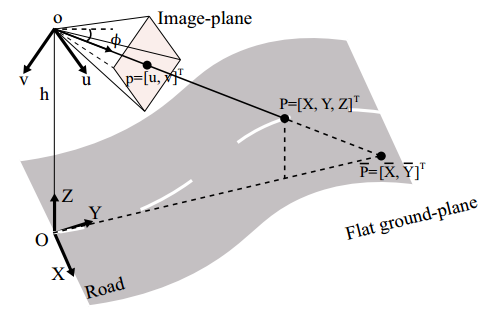
\includegraphics[width=9cm, height=5cm]{images/3d_lane_geometry.png}
    \caption{Geometric representation of lane point in 3D world space, image plane and virtual top view \cite{DBLP:journals/corr/abs-2112-15351}}
    \end{figure}
    
    In the above figure the point $\textbf{P} =[X, Y, Z]^{T}$ is in 3D space and when it is projected onto the image plane it is defined by $\textbf{p} = [u, v]^{T}$. Birds eye view can be seen as the projection of point $\textbf{P}$ from 3D space to flat ground plane, where $Z=0$. $\textbf{O}$ is the origin of the 3D space which is obtained by projecting the origin of camera center $\textbf{o}$ on to the flat ground plane with $Z = 0$. The focal length and other intrinsic parameters of the camera is fixed, where as the orientation of the camera in terms of camera height \textbf{h}  and camera pitch \textbf{$\phi$} is fixed or sometimes it is predicted from the network. 
    
    Using geometric transformation and homography as discussed above we can project points in 3D space to virtual flat ground plane. As per the figure 4.1 we can say that the point \textbf{P} it projection on image plane and flat ground plane, all lies on the same ray and this co-linear relationship will hold even if when there are downhill scenarios where $Z<0$. 
    
      \begin{figure}[h]
    \centering
    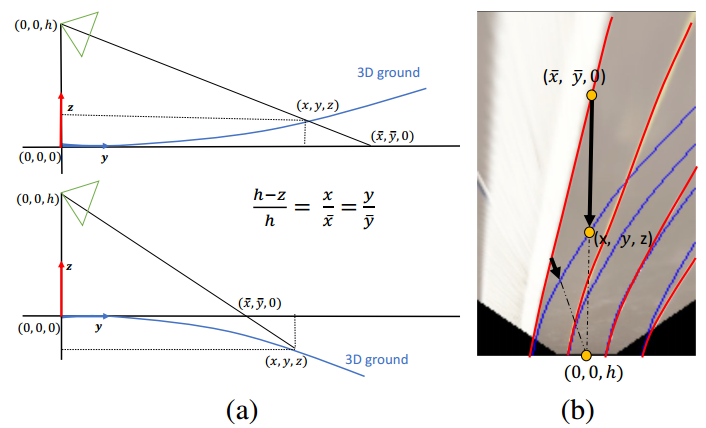
\includegraphics[width=9cm, height=5cm]{images/collinear_3dlane.png}
    \caption{Another view of the co-linear relationship between the 3D lane points $(x,y,z)$, its projection on virtual top view $(\overline{x}, \overline{y},0)$ and camera center $(0,0,h)$ \cite{guo2020gen}}
    \end{figure}

    Therefore we can obtain a relationship between the points from 3d world to virtual top view as :
    \begin{center}
        $\frac{h-z}{h} =\frac{x}{\overline{x}}=\frac{y}{\overline{y}}$ 
    \end{center}
    
    using the above formulation we can represent this transformation from 3D world space to virtual top view as \textbf{$\overline{P} = GP$}, where \textbf{G} is the transformation matrix. Similarly a point \textbf{$\overline{P}$} can be projected onto the image plane as $\textbf{p}$ using homomgraphy which is also discussed in section 2.2. and this can be represented as: 
    \begin{center}
       $\begin{bmatrix}\overline{u}  \\\overline{v} \\ \overline{z}\end{bmatrix} = \begin{bmatrix} f_{x} & 0& c_{x}  \\0 &f_{x} & c_{y} \\ 0 & 0 & 1     \end{bmatrix}\begin{bmatrix} 1 & 0& 0  \\0 &cos(\phi+ \frac{\theta}{2}) & h \\ 0 &cos(\phi+ \frac{\theta}{2}) & 0     \end{bmatrix}\begin{bmatrix}\overline{X}  \\\overline{Y} \\ 1\end{bmatrix}$
    \end{center}

    Here, \textbf{$\widetilde{p}$} $= (\widetilde{u}, \widetilde{v}, \widetilde{z})$ and  \textbf{$\widetilde{P}$} $= (\overline{X},\overline{Y},1 )$ are represented in the form of homogeneous coordinates, therefore $u = \frac{\widetilde{u}} {\widetilde{z}} $ and $v = \frac{\widetilde{v}} {\widetilde{z}} $. Similar as above this can be represented as \textbf{$\widetilde{p} = H\widetilde{P}$}, where H is the homography transformation matrix. 
    
    \subsection{Anchor Representation of lane line points}
    Some of the approaches used in this work are predicting 3D lane line points in the from of anchors and even the ground-truth points are also converted in the form of anchors as target tensors to the network.  As per the 3D lane geometry discussed above, x is the lateral axes and Y is the forward axes with respect to a scene. These anchors are generally predefined on the basis of  equally spaced distance in x and y directions. 
    
     \begin{figure}[h]
    \centering
    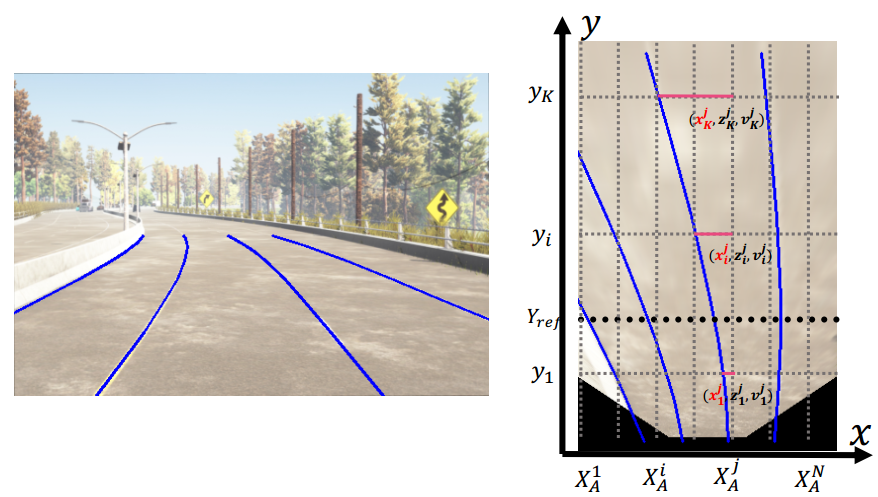
\includegraphics[width=9cm, height=5cm]{images/anchor_3Dlane.png}
    \caption{Lane anchor representation \cite{guo2020gen}}
    \end{figure}
    
    As per the figure 4.3, there exist N lane anchors (Vertical lines) in terms of N equally spaced position in X-direction ($X^{i}_{A}$)$^{N}_{i=1}$. The position on anchors in y-direction can be equally spaced or on the basis of certain distances in the forward direction. Therefore a 3D lane line in this can be represented by an anchor $X^{i}_{A}$ where each anchor contains $3*K$ attributes. K is the number of steps in y-direction. So at each step $(Y_ref)$ ground-truth lane anchor attributes ($\overline{x}^{i}_{j},z^{i}_{j},v^{i}_{j}$)$^{K}_{j=1}$ are calculated by associating it with the closest distance in x-direction. 
        
        \subsection{Architecture: 1}
        
        \subsection{Architecture: 2}
        \subsubsection{Stage 1: Image Segmentation}
        \subsubsection{Stage 2: Semi-Local 3D Lane Detection}
    
    \subsection{Loss Functions}
        (Write in general mentioning the sections which loss functions is used for what)
        
    \subsection{Experimental setup}
        \subsubsection{Datasets Used}
        \subsubsection{Evaluation Metrics}
        \subsubsection{Implementation Details}
    
    \section{Pipeline Workflow: 3D Lane AuxNet}
        \subsection{Architecture}
        \subsection{Dataset Used}
        \subsection{Evaluation Metrics}
        \subsection{Implementation Details}
        
\end{document}
